% Intended LaTeX compiler: xelatex
\documentclass[a4paper, 12pt]{article}
\usepackage{graphicx}
\usepackage{longtable}
\usepackage{wrapfig}
\usepackage{rotating}
\usepackage[normalem]{ulem}
\usepackage{amsmath}
\usepackage{amssymb}
\usepackage{capt-of}
\usepackage{hyperref}
\usepackage[danish]{babel}
\usepackage{mathtools}
\usepackage[margin=3.0cm]{geometry}
\hypersetup{colorlinks, linkcolor=black, urlcolor=blue}
\setlength{\parindent}{0em}
\parskip 1.5ex
\author{Jacob Debel}
\date{Fysik B}
\title{Elektromotorisk kraft \& indre modstand\\\medskip
\large Elektricitet}
\hypersetup{
 pdfauthor={Jacob Debel},
 pdftitle={Elektromotorisk kraft \& indre modstand},
 pdfkeywords={},
 pdfsubject={},
 pdfcreator={Emacs 29.4 (Org mode 9.6.15)}, 
 pdflang={Danish}}
\begin{document}

\maketitle

\section*{Motivation}
\label{sec:orgbc3f3c3}
Når vi har talt om spændingskilder/batterier, har vi typisk antaget at deres spænding er konstant og således udfører et konstant arbejde per ladning. Dette er dog \textbf{ikke} sandt i virkeligheden.
Tænk på, hvis der skulle trækkes en (uendelige) stor strøm, så skulle batteriet kunne udføre et (uendeligt) stort arbejde. Dette giver komplikationer med loven om energibevarelse.
I stedet har det vist sig, at hvis man forsøget at trække en stor strøm ud af et batteri, så falder \emph{polspændingen} (altså spændingen over batteripolerne og dermed også over det tilsluttede kredsløb).

\section*{Teori}
\label{sec:orgddadf50}
For at beskrive det føromtalte fald i spænding som funktion af strømmen, defineres den elektromotoriske kraft ( emk, \(\epsilon\), \(U_0\)) som polspændingen når der løber en uendelig lille strøm.
En fysisk spændingsforsyning kan da teoretisk betragtes som en seriekobling af en \textbf{superspændingskilde}, som altid yder en spænding på \(U_0\) og så en modstand \(R_i\) som kaldes den \textbf{indre modstand}.
Forbindes spændingsforsyningen nu til en ydre modstand med resistansen \(R_y\), så siger Ohms lov

$$U_0 = R_i \cdot I + R_y \cdot I\,.$$

Dog er \(R_y \cdot I=U_p\), hvor \(U_P\) er polspændingen og ovenstående ligning kan omskrives til:

\begin{align*}
U_0 &= R_i \cdot I + U_p \iff \\
U_p &= U_0 - R_i \cdot I \,.
\end{align*}

Altså vil polspændingen falde som funktion af strømmen.

Det er denne sammenhæng, I skal undersøge i dette forsøg.

\textbf{I skal indsamle data, så vi senere kan bestemme den indre modstand \(R_i\) , kortslutningsstrømmen \(I_{maks}\) og den elektromotoriske kraft for forskellige almindelige 9 V batterier.}

\section*{Udstyr}
\label{sec:orgaf0e26f}
\begin{itemize}
\item 1 voltmeter (multimeter sat til at måle spænding)
\item 2 skydepotentiometre/variable modstande (på hhv. \(1-10 \Omega\) og \(100-1000 \Omega\).)
\item Diverse nye og gamle(brugte) 9V-batterier.
\end{itemize}

\section*{Fremgangsmåde}
\label{sec:org30d2f47}
\begin{enumerate}
\item Opstil følgende kredsløb (se bort fra amperemeteret. Strømmen kan I beregne i stedet):

\begin{center}
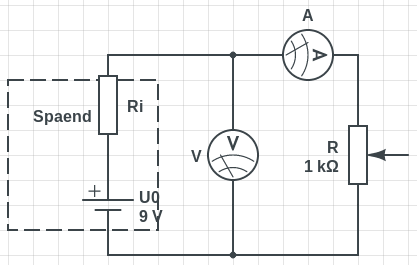
\includegraphics[width=.9\linewidth]{./img/kredsloeb.png}
\end{center}

\item Til de nye 9V-batterier benyttes potentiometeret på \(1-10 \Omega\) og til de gamle benyttes \(100-1000 \Omega\). Fælles for begge forsøgsopstillinger er at potentiometeret skal starte med at være på den største mulige modstand.

\item Ændr nu på den variable modstand \(R\) og notér sammenhørende værdier af \(U\) og \(R\).

Beregn her ud fra yderligere strømmen gennem den ydre modstand, \(I\).

Optag ca. 10 målinger jævnt fordelt mellem tomgang og kortsluttet tilstand. \textbf{I må dog ikke kortslutte batterierne!!!}
\end{enumerate}
\section*{Databehandling}
\label{sec:orga8edf8d}
\begin{itemize}
\item Indsæt måleresultaterne i et regneark og generer for hvert batteri et plot med \(I\) ud af 1. aksen og \(U\) op ad 2. aksen.
\item Batteriernes indre modstand kan på en eller anden måde bestemmes ud fra disse plots. Det må I/vi lige tænke os til. Sammen skal vi nok komme frem til noget smart. :)
\end{itemize}
\end{document}
